% Options for packages loaded elsewhere
\PassOptionsToPackage{unicode}{hyperref}
\PassOptionsToPackage{hyphens}{url}
%
\documentclass[
]{article}
\usepackage{amsmath,amssymb}
\usepackage{iftex}
\ifPDFTeX
  \usepackage[T1]{fontenc}
  \usepackage[utf8]{inputenc}
  \usepackage{textcomp} % provide euro and other symbols
\else % if luatex or xetex
  \usepackage{unicode-math} % this also loads fontspec
  \defaultfontfeatures{Scale=MatchLowercase}
  \defaultfontfeatures[\rmfamily]{Ligatures=TeX,Scale=1}
\fi
\usepackage{lmodern}
\ifPDFTeX\else
  % xetex/luatex font selection
\fi
% Use upquote if available, for straight quotes in verbatim environments
\IfFileExists{upquote.sty}{\usepackage{upquote}}{}
\IfFileExists{microtype.sty}{% use microtype if available
  \usepackage[]{microtype}
  \UseMicrotypeSet[protrusion]{basicmath} % disable protrusion for tt fonts
}{}
\makeatletter
\@ifundefined{KOMAClassName}{% if non-KOMA class
  \IfFileExists{parskip.sty}{%
    \usepackage{parskip}
  }{% else
    \setlength{\parindent}{0pt}
    \setlength{\parskip}{6pt plus 2pt minus 1pt}}
}{% if KOMA class
  \KOMAoptions{parskip=half}}
\makeatother
\usepackage{xcolor}
\usepackage[margin=1in]{geometry}
\usepackage{color}
\usepackage{fancyvrb}
\newcommand{\VerbBar}{|}
\newcommand{\VERB}{\Verb[commandchars=\\\{\}]}
\DefineVerbatimEnvironment{Highlighting}{Verbatim}{commandchars=\\\{\}}
% Add ',fontsize=\small' for more characters per line
\usepackage{framed}
\definecolor{shadecolor}{RGB}{248,248,248}
\newenvironment{Shaded}{\begin{snugshade}}{\end{snugshade}}
\newcommand{\AlertTok}[1]{\textcolor[rgb]{0.94,0.16,0.16}{#1}}
\newcommand{\AnnotationTok}[1]{\textcolor[rgb]{0.56,0.35,0.01}{\textbf{\textit{#1}}}}
\newcommand{\AttributeTok}[1]{\textcolor[rgb]{0.13,0.29,0.53}{#1}}
\newcommand{\BaseNTok}[1]{\textcolor[rgb]{0.00,0.00,0.81}{#1}}
\newcommand{\BuiltInTok}[1]{#1}
\newcommand{\CharTok}[1]{\textcolor[rgb]{0.31,0.60,0.02}{#1}}
\newcommand{\CommentTok}[1]{\textcolor[rgb]{0.56,0.35,0.01}{\textit{#1}}}
\newcommand{\CommentVarTok}[1]{\textcolor[rgb]{0.56,0.35,0.01}{\textbf{\textit{#1}}}}
\newcommand{\ConstantTok}[1]{\textcolor[rgb]{0.56,0.35,0.01}{#1}}
\newcommand{\ControlFlowTok}[1]{\textcolor[rgb]{0.13,0.29,0.53}{\textbf{#1}}}
\newcommand{\DataTypeTok}[1]{\textcolor[rgb]{0.13,0.29,0.53}{#1}}
\newcommand{\DecValTok}[1]{\textcolor[rgb]{0.00,0.00,0.81}{#1}}
\newcommand{\DocumentationTok}[1]{\textcolor[rgb]{0.56,0.35,0.01}{\textbf{\textit{#1}}}}
\newcommand{\ErrorTok}[1]{\textcolor[rgb]{0.64,0.00,0.00}{\textbf{#1}}}
\newcommand{\ExtensionTok}[1]{#1}
\newcommand{\FloatTok}[1]{\textcolor[rgb]{0.00,0.00,0.81}{#1}}
\newcommand{\FunctionTok}[1]{\textcolor[rgb]{0.13,0.29,0.53}{\textbf{#1}}}
\newcommand{\ImportTok}[1]{#1}
\newcommand{\InformationTok}[1]{\textcolor[rgb]{0.56,0.35,0.01}{\textbf{\textit{#1}}}}
\newcommand{\KeywordTok}[1]{\textcolor[rgb]{0.13,0.29,0.53}{\textbf{#1}}}
\newcommand{\NormalTok}[1]{#1}
\newcommand{\OperatorTok}[1]{\textcolor[rgb]{0.81,0.36,0.00}{\textbf{#1}}}
\newcommand{\OtherTok}[1]{\textcolor[rgb]{0.56,0.35,0.01}{#1}}
\newcommand{\PreprocessorTok}[1]{\textcolor[rgb]{0.56,0.35,0.01}{\textit{#1}}}
\newcommand{\RegionMarkerTok}[1]{#1}
\newcommand{\SpecialCharTok}[1]{\textcolor[rgb]{0.81,0.36,0.00}{\textbf{#1}}}
\newcommand{\SpecialStringTok}[1]{\textcolor[rgb]{0.31,0.60,0.02}{#1}}
\newcommand{\StringTok}[1]{\textcolor[rgb]{0.31,0.60,0.02}{#1}}
\newcommand{\VariableTok}[1]{\textcolor[rgb]{0.00,0.00,0.00}{#1}}
\newcommand{\VerbatimStringTok}[1]{\textcolor[rgb]{0.31,0.60,0.02}{#1}}
\newcommand{\WarningTok}[1]{\textcolor[rgb]{0.56,0.35,0.01}{\textbf{\textit{#1}}}}
\usepackage{longtable,booktabs,array}
\usepackage{calc} % for calculating minipage widths
% Correct order of tables after \paragraph or \subparagraph
\usepackage{etoolbox}
\makeatletter
\patchcmd\longtable{\par}{\if@noskipsec\mbox{}\fi\par}{}{}
\makeatother
% Allow footnotes in longtable head/foot
\IfFileExists{footnotehyper.sty}{\usepackage{footnotehyper}}{\usepackage{footnote}}
\makesavenoteenv{longtable}
\usepackage{graphicx}
\makeatletter
\def\maxwidth{\ifdim\Gin@nat@width>\linewidth\linewidth\else\Gin@nat@width\fi}
\def\maxheight{\ifdim\Gin@nat@height>\textheight\textheight\else\Gin@nat@height\fi}
\makeatother
% Scale images if necessary, so that they will not overflow the page
% margins by default, and it is still possible to overwrite the defaults
% using explicit options in \includegraphics[width, height, ...]{}
\setkeys{Gin}{width=\maxwidth,height=\maxheight,keepaspectratio}
% Set default figure placement to htbp
\makeatletter
\def\fps@figure{htbp}
\makeatother
\setlength{\emergencystretch}{3em} % prevent overfull lines
\providecommand{\tightlist}{%
  \setlength{\itemsep}{0pt}\setlength{\parskip}{0pt}}
\setcounter{secnumdepth}{-\maxdimen} % remove section numbering
\usepackage{booktabs}
\usepackage{longtable}
\usepackage{array}
\usepackage{multirow}
\usepackage{wrapfig}
\usepackage{float}
\usepackage{colortbl}
\usepackage{pdflscape}
\usepackage{tabu}
\usepackage{threeparttable}
\usepackage{threeparttablex}
\usepackage[normalem]{ulem}
\usepackage{makecell}
\usepackage{xcolor}
\ifLuaTeX
  \usepackage{selnolig}  % disable illegal ligatures
\fi
\usepackage[]{natbib}
\bibliographystyle{plainnat}
\usepackage{bookmark}
\IfFileExists{xurl.sty}{\usepackage{xurl}}{} % add URL line breaks if available
\urlstyle{same}
\hypersetup{
  pdftitle={PEC1 - Análisis de Datos Ómicos},
  pdfauthor={Lidia Getino Álvarez},
  hidelinks,
  pdfcreator={LaTeX via pandoc}}

\title{PEC1 - Análisis de Datos Ómicos}
\usepackage{etoolbox}
\makeatletter
\providecommand{\subtitle}[1]{% add subtitle to \maketitle
  \apptocmd{\@title}{\par {\large #1 \par}}{}{}
}
\makeatother
\subtitle{Curso 2024-2025}
\author{Lidia Getino Álvarez}
\date{6 de noviembre, 2024}

\begin{document}
\maketitle

{
\setcounter{tocdepth}{3}
\tableofcontents
}
\section{1. Introducción}\label{introducciuxf3n}

\subsection{1.1. Resumen}\label{resumen}

El presente informe recoge una propuesta de solución a la primera prueba
de evaluación contínua (PEC) de la asignatura \emph{Análisis de Datos
Ómicos}.

A lo largo de este, se ha trabajado con un conjunto de datos de
metabolómica, sobre el cual se han aplicado las herramientas
bioinformáticas y estadísticas necesarias para llevar a cabo una
exploración del mismo:

\begin{itemize}
\item
  En primer lugar, se ha mostrado el proceso de selección e importación
  de los datos en \emph{RStudio}.
\item
  A continuación, se ha realizado una exploración inicial del conjunto
  de datos con la finalidad de familiarizarse con su estructura e
  información.
\item
  Finalmente, se ha planteado una pregunta de interés biológico y se ha
  resuelto aplicando las técnicas estadísticas que se han considerado
  más apropiadas.
\end{itemize}

\subsection{1.2. Objetivos}\label{objetivos}

El objetivo principal de este trabajo consiste en llevar a cabo un
análisis exploratorio de un conjunto de datos metabolómicos, aplicando
un contenedor de tipo \emph{SummarizedExperiment}, perteneciente al
conjunto de paquetes de \emph{Bioconductor}.

Como objetivos secundarios se encuentran la familiarización con los
datos de experimetos metabolómicos y el manejo de repositorios
colaboratorivos con control de versiones (\emph{github}).

Adicionalmente, como parte de la exploración de los datos, se planteará
una pregunta biológica apropiada a la naturaleza de los datos con los
que se trabaje y se intentará responder empleando los métodos
estadísticos que se consideren más apropiados para ello.

\section{2. Materiales y métodos}\label{materiales-y-muxe9todos}

\subsection{2.1. Conjunto de datos de
trabajo}\label{conjunto-de-datos-de-trabajo}

El conjunto de datos empleado se ha obtenido del repositorio de datos de
metabolómica \emph{Metabolomics Workbench}
(\url{https://www.metabolomicsworkbench.org/}). Para la selección, se
realizó una breve revisión de los estudios disponibles en la mencionada
base de datos y se escogió uno en función de su temática y el interés
del mismo: \textbf{\emph{ST002787 - Metabolomic analysis of gut
metabolites in colorectal cancer patients: correlation with disease
development and outcome}}, perteneciente al proyecto con ID: PR001737
\citep{PR001737}.

En este estudio de la \emph{Wuhan University of Science and Technology},
los investigadores llevaron a cabo un análisis exploratorio del perfil
metabolómico de las muestras fecales de 35 pacientes de cáncer
colorectal, 37 pacientes de adenoma colorrectal y 30 pacientes sanos,
con el objetivo de determinar posibles biomarcadores metabolómicos que
diferenciasen a los tres grupos.

La recolección de las muestras fecales se llevó a cabo en pacientes que
se sometieron a una colonoscopia y a un examen histopatológico en el
Hospital Tianyou (Wuhan, China). A continuación, estas se prepararon y
se sometieron a un análisis de espectrometría de masas en tándem por
cromatografía líquida (LC-MS/MS). Finalmente, para la busqueda de
potenciales biomarcadores, aplicaron técnicas de análisis estadístico,
como el \emph{Orthogonal Partial Least Squares Discriminant Analysis}
(OPLS-DA) o el \emph{Receiver operating characteristic Analysis} (ROC).

\subsection{2.2. Métodos y herramientas bioinformáticas
utilizados}\label{muxe9todos-y-herramientas-bioinformuxe1ticas-utilizados}

Para la realización de este trabajo, se ha empleado el entorno de
desarrollo integrado (IDE) \emph{RStudio} \citep{RStudio}, el cual
proporciona una interfaz cómoda para la programación en lenguaje
\emph{R} y la redacción de infórmes dinámicos con \emph{RMarkdown}.

La importación y exploración inicial del conjunto de datos se ha llevado
a cabo empleando algunas de las librerías del proyecto Bioconductor
\citep{Bioconductor}, concretamente \emph{metabolomicsWorkbenchR},
\emph{SummarizedExperiment} y \emph{mixOmmics}.

Finalmente, como parte del proceso de exploración, se ha planteado una
pregunta biológica de interés y se ha resuelto aplicando técnicas de
análisis estadístico como el \emph{Principal components analysis} (PCA)
o el método de \emph{Partial Least Squares Discriminant Analysis}
(PLS-DA), cuya relevancia y motivo de selección se especificará a lo
largo del informe.

\subsection{\texorpdfstring{2.3. Repositorio en
\emph{github}}{2.3. Repositorio en github}}\label{repositorio-en-github}

El presente informe, así como los archivos asociados al mismo, se
alojarán en un repositorio público en el servicio web de repositorios
con control de versiones, \emph{github} \citep{github}. Para ello, se ha
creado el repositorio en la web de \emph{github} y, a continuación, se
ha abierto un proyecto con control de versiones en \emph{RStudio}, al
cual se le ha proporcionado la URL del repositorio previamente creado,
quedando así enlazados.

\section{3. Resultados}\label{resultados}

\subsection{3.1. Obtención de los datos y creación del
contenedor}\label{obtenciuxf3n-de-los-datos-y-creaciuxf3n-del-contenedor}

Una vez seleccionado el conjunto de datos, se procede a su importación
en \emph{R}, empleando la función \emph{do\_query()} del paquete
\emph{metabolomicsWorkbenchR}. Esta función permite realizar una
consulta directa en \emph{Metabolomics Workbench} e importar los datos
de un estudio como un objeto de clase \emph{SummarizedExperiment}.

\begin{Shaded}
\begin{Highlighting}[]
\CommentTok{\# Realizo una consulta para acceder a los datos del estudio ST002787}
\NormalTok{se\_data }\OtherTok{\textless{}{-}} \FunctionTok{do\_query}\NormalTok{(}
  \CommentTok{\# Tipo de busqueda: por estudio}
  \AttributeTok{context =} \StringTok{\textquotesingle{}study\textquotesingle{}}\NormalTok{,}
  \CommentTok{\# Dato proporcionado para la búsqueda: ID del estudio}
  \AttributeTok{input\_item =} \StringTok{\textquotesingle{}study\_id\textquotesingle{}}\NormalTok{,}
  \CommentTok{\# ID del estudio}
  \AttributeTok{input\_value =} \StringTok{\textquotesingle{}ST002787\textquotesingle{}}\NormalTok{,}
  \CommentTok{\# Tipo de datos de salida: SummarizedExperiment}
  \AttributeTok{output\_item =} \StringTok{\textquotesingle{}SummarizedExperiment\textquotesingle{}}
\NormalTok{)}

\CommentTok{\# Observo el output de la consulta}
\NormalTok{se\_data}
\end{Highlighting}
\end{Shaded}

\begin{verbatim}
## $AN004534
## class: SummarizedExperiment 
## dim: 1074 102 
## metadata(8): data_source study_id ... description subject_type
## assays(1): ''
## rownames(1074): ME723397 ME722671 ... ME723400 ME722714
## rowData names(3): metabolite_name metabolite_id refmet_name
## colnames(102): CRA001 CRA002 ... HC029 HC030
## colData names(7): local_sample_id study_id ... Group_type Sex
## 
## $AN004535
## class: SummarizedExperiment 
## dim: 567 102 
## metadata(8): data_source study_id ... description subject_type
## assays(1): ''
## rownames(567): ME723973 ME723992 ... ME723784 ME723808
## rowData names(3): metabolite_name metabolite_id refmet_name
## colnames(102): CRA001 CRA002 ... HC029 HC030
## colData names(7): local_sample_id study_id ... Group_type Sex
\end{verbatim}

A primera vista, se observa que los datos importados del estudio
\emph{ST002787} se conforman de dos objetos de la clase
\emph{SummarizedExperiment}, pertenecientes a dos análisis diferentes.
Estos parecen compartir formato, aunque no dimensiones, pues uno de
ellos (AN004534) consta de 1074 filas (o metabolitos detectados) y el
otro (AN004535) de 567. En los siguientes apartados profundizaremos más
en las carácterísticas de estos datos.

\subsubsection{\texorpdfstring{3.1.1. Ejemplo de creación de un
contenedor \emph{SummarizedExperiment} desde
cero}{3.1.1. Ejemplo de creación de un contenedor SummarizedExperiment desde cero}}\label{ejemplo-de-creaciuxf3n-de-un-contenedor-summarizedexperiment-desde-cero}

Inicialmente, por una mala interpretación del enunciado del trabajo,
realicé la importación de los datos directamente en formato
\emph{SummarizedExperiment} desde \emph{Metabolomics Workbench}, como se
ha demostrado previamente. Sin embargo, tras recibir una comunicación
aclaratoria en el foro de la asignatura, entendí que parte del interés
del trabajo consistía en transformar, nosotros mismos, unos datos de
partida en formato matriz a un contenedor de tipo
\emph{SummarizedExperiment}.

Dado que en el momento de la recepción de dicho anuncio ya había
avanzado con el resto de los ejercicios propuestos usando el conjunto de
datos arriba mencionado, tomé la decisión de centrar mi trabajo en dicho
conjunto. No obstante, muestro a continuación un ejemplo de creación de
un contenedor \emph{SummarizedExperiment} a partir de uno de los
conjuntos de datos del repositorio de \emph{github} proporcionado en el
enunciado: \emph{human\_cachexia.csv}.

En primer lugar, cargo el archivo de datos en \emph{R} y visualizo su
estructura:

\begin{Shaded}
\begin{Highlighting}[]
\CommentTok{\# Cargo el archivo y guardo sus dimensiones}
\NormalTok{cachexia\_data }\OtherTok{\textless{}{-}} \FunctionTok{read.csv}\NormalTok{(}\StringTok{"human\_cachexia.csv"}\NormalTok{, }\AttributeTok{stringsAsFactors =} \ConstantTok{FALSE}\NormalTok{)}
\NormalTok{dim\_cachexia }\OtherTok{\textless{}{-}} \FunctionTok{dim}\NormalTok{(cachexia\_data)}

\CommentTok{\# Muestro de forma resumida la estructura del archivo}
\FunctionTok{str}\NormalTok{(cachexia\_data, }\AttributeTok{list.len =} \DecValTok{5}\NormalTok{)}
\end{Highlighting}
\end{Shaded}

\begin{verbatim}
## 'data.frame':    77 obs. of  65 variables:
##  $ Patient.ID                 : chr  "PIF_178" "PIF_087" "PIF_090" "NETL_005_V1" ...
##  $ Muscle.loss                : chr  "cachexic" "cachexic" "cachexic" "cachexic" ...
##  $ X1.6.Anhydro.beta.D.glucose: num  40.9 62.2 270.4 154.5 22.2 ...
##  $ X1.Methylnicotinamide      : num  65.4 340.4 64.7 53 73.7 ...
##  $ X2.Aminobutyrate           : num  18.7 24.3 12.2 172.4 15.6 ...
##   [list output truncated]
\end{verbatim}

Vemos que el conjunto de datos consta de 77 observaciones, o pacientes,
y 65 variables, entre las cuales tenemos el ID del paciente
(\emph{Patient.ID}), la variable de identificación del grupo del
paciente en función de si padece o no cachexia (\emph{Muscle.loss}) y
una serie de metabolitos analizados.

Para estructurar el contenedor de tipo \emph{SummarizedExperiment}, voy
a crear los siguientes elementos propios de la clase:

\begin{itemize}
\tightlist
\item
  \textbf{Assay}: se compone de la matriz de datos principal, con los
  elementos biológicos de interés en las filas y las muestras, o
  pacientes, en las columnas. Por tanto, esta matriz la crearé
  trasponiendo el conjunto de datos original y eliminando las dos
  primeras columnas, para dejar así solo las columnas referentes a los
  metabolitos.
\end{itemize}

\begin{Shaded}
\begin{Highlighting}[]
\CommentTok{\# Antes de nada, asigno a las filas del conjunto el nombre del ID de paciente}
\FunctionTok{rownames}\NormalTok{(cachexia\_data) }\OtherTok{\textless{}{-}}\NormalTok{ cachexia\_data}\SpecialCharTok{$}\NormalTok{Patient.ID}

\CommentTok{\# Creo el assay con el conjunto original traspuesto, eliminado las dos primeras columnas}
\NormalTok{n\_col }\OtherTok{\textless{}{-}}\NormalTok{ dim\_cachexia[}\DecValTok{2}\NormalTok{] }\CommentTok{\#nº de columnas}
\NormalTok{cachexia\_assay }\OtherTok{\textless{}{-}} \FunctionTok{t}\NormalTok{(cachexia\_data[,}\DecValTok{3}\SpecialCharTok{:}\NormalTok{n\_col])}

\CommentTok{\# Muestro unos pocos registros del assay generado}
\FunctionTok{kable}\NormalTok{(}\FunctionTok{head}\NormalTok{(cachexia\_assay[,}\DecValTok{1}\SpecialCharTok{:}\DecValTok{5}\NormalTok{],}\DecValTok{4}\NormalTok{))}
\end{Highlighting}
\end{Shaded}

\begin{longtable}[]{@{}
  >{\raggedright\arraybackslash}p{(\columnwidth - 10\tabcolsep) * \real{0.3889}}
  >{\raggedleft\arraybackslash}p{(\columnwidth - 10\tabcolsep) * \real{0.1111}}
  >{\raggedleft\arraybackslash}p{(\columnwidth - 10\tabcolsep) * \real{0.1111}}
  >{\raggedleft\arraybackslash}p{(\columnwidth - 10\tabcolsep) * \real{0.1111}}
  >{\raggedleft\arraybackslash}p{(\columnwidth - 10\tabcolsep) * \real{0.1667}}
  >{\raggedleft\arraybackslash}p{(\columnwidth - 10\tabcolsep) * \real{0.1111}}@{}}
\toprule\noalign{}
\begin{minipage}[b]{\linewidth}\raggedright
\end{minipage} & \begin{minipage}[b]{\linewidth}\raggedleft
PIF\_178
\end{minipage} & \begin{minipage}[b]{\linewidth}\raggedleft
PIF\_087
\end{minipage} & \begin{minipage}[b]{\linewidth}\raggedleft
PIF\_090
\end{minipage} & \begin{minipage}[b]{\linewidth}\raggedleft
NETL\_005\_V1
\end{minipage} & \begin{minipage}[b]{\linewidth}\raggedleft
PIF\_115
\end{minipage} \\
\midrule\noalign{}
\endhead
\bottomrule\noalign{}
\endlastfoot
X1.6.Anhydro.beta.D.glucose & 40.85 & 62.18 & 270.43 & 154.47 & 22.20 \\
X1.Methylnicotinamide & 65.37 & 340.36 & 64.72 & 52.98 & 73.70 \\
X2.Aminobutyrate & 18.73 & 24.29 & 12.18 & 172.43 & 15.64 \\
X2.Hydroxyisobutyrate & 26.05 & 41.68 & 65.37 & 74.44 & 83.93 \\
\end{longtable}

\begin{itemize}
\tightlist
\item
  \textbf{colData}: consiste en los metadatos adicionales referentes a
  las muestras del experimento. En este caso, los metadatos de las
  muestras se compondrían de las dos primeras columnas del archivo de
  datos original, pues no disponemos de más información al respecto.
\end{itemize}

\begin{Shaded}
\begin{Highlighting}[]
\CommentTok{\# Creo el DataFrame de colData con las dos primeras columnas del conjunto original}
\NormalTok{cachexia\_colData }\OtherTok{\textless{}{-}} \FunctionTok{DataFrame}\NormalTok{(cachexia\_data[,}\DecValTok{1}\SpecialCharTok{:}\DecValTok{2}\NormalTok{])}

\CommentTok{\# Muestro unos pocos registros del colData generado}
\FunctionTok{kable}\NormalTok{(}\FunctionTok{head}\NormalTok{(}\FunctionTok{as.data.frame}\NormalTok{(cachexia\_colData),}\DecValTok{4}\NormalTok{))}
\end{Highlighting}
\end{Shaded}

\begin{longtable}[]{@{}lll@{}}
\toprule\noalign{}
& Patient.ID & Muscle.loss \\
\midrule\noalign{}
\endhead
\bottomrule\noalign{}
\endlastfoot
PIF\_178 & PIF\_178 & cachexic \\
PIF\_087 & PIF\_087 & cachexic \\
PIF\_090 & PIF\_090 & cachexic \\
NETL\_005\_V1 & NETL\_005\_V1 & cachexic \\
\end{longtable}

\begin{itemize}
\tightlist
\item
  \textbf{rowData}: consiste en los metadatos adicionales referentes a
  los elementos biológicos de interés. En este caso, los elementos
  biológicos de interés son los metabolitos, de los cuales solo
  conocemos el nombre. Por tanto, solo contendrá una columna con el
  nombre de los mismos.
\end{itemize}

\begin{Shaded}
\begin{Highlighting}[]
\CommentTok{\# Creo el DataFrame de rowData con los nombres de los metabolitos}
\NormalTok{met\_names }\OtherTok{\textless{}{-}} \FunctionTok{colnames}\NormalTok{(cachexia\_data[,}\DecValTok{3}\SpecialCharTok{:}\NormalTok{n\_col])}
\NormalTok{cachexia\_rowData }\OtherTok{\textless{}{-}} \FunctionTok{DataFrame}\NormalTok{(}\AttributeTok{Metabolites =}\NormalTok{ met\_names, }\AttributeTok{row.names =}\NormalTok{ met\_names)}

\CommentTok{\# Muestro unos pocos registros del colData generado}
\FunctionTok{kable}\NormalTok{(}\FunctionTok{head}\NormalTok{(}\FunctionTok{as.data.frame}\NormalTok{(cachexia\_rowData),}\DecValTok{4}\NormalTok{))}
\end{Highlighting}
\end{Shaded}

\begin{longtable}[]{@{}ll@{}}
\toprule\noalign{}
& Metabolites \\
\midrule\noalign{}
\endhead
\bottomrule\noalign{}
\endlastfoot
X1.6.Anhydro.beta.D.glucose & X1.6.Anhydro.beta.D.glucose \\
X1.Methylnicotinamide & X1.Methylnicotinamide \\
X2.Aminobutyrate & X2.Aminobutyrate \\
X2.Hydroxyisobutyrate & X2.Hydroxyisobutyrate \\
\end{longtable}

A continuación, procedo a la constitución del contenedor a partir de los
elementos recién creados:

\begin{Shaded}
\begin{Highlighting}[]
\CommentTok{\# Aplico la función SummarizedExperiment()}
\NormalTok{cachexia\_se }\OtherTok{\textless{}{-}} \FunctionTok{SummarizedExperiment}\NormalTok{(}
  \AttributeTok{assays =} \FunctionTok{list}\NormalTok{(}\AttributeTok{counts =}\NormalTok{ cachexia\_assay),}
  \AttributeTok{rowData =}\NormalTok{ cachexia\_rowData,}
  \AttributeTok{colData =}\NormalTok{ cachexia\_colData}
\NormalTok{)}

\NormalTok{cachexia\_se}
\end{Highlighting}
\end{Shaded}

\begin{verbatim}
## class: SummarizedExperiment 
## dim: 63 77 
## metadata(0):
## assays(1): counts
## rownames(63): X1.6.Anhydro.beta.D.glucose X1.Methylnicotinamide ...
##   pi.Methylhistidine tau.Methylhistidine
## rowData names(1): Metabolites
## colnames(77): PIF_178 PIF_087 ... NETL_003_V1 NETL_003_V2
## colData names(2): Patient.ID Muscle.loss
\end{verbatim}

Como se puede observar, el conjunto de datos \emph{human\_cachexia.csv}
está ahora correctamente formateado en forma de objeto
\emph{SummarizedExperiment}.

Visto este ejemplo, el resto del informe, como mencioné anteriormente,
está realizado con el conjunto de datos importado directamente desde
\emph{Metabolomics Workbench}.

\subsection{3.2. Exploración de los
datos}\label{exploraciuxf3n-de-los-datos}

\subsubsection{3.2.1. Observación de los
metadatos}\label{observaciuxf3n-de-los-metadatos}

Como punto de partida, se explora la información experimental de cada
análisis del conjunto de datos con el fin de determinar las diferencias
entre ambos. Esta información es accesible mediante la función
\emph{metadata()} del paquete \emph{SummarizedExperiment}.

\begin{Shaded}
\begin{Highlighting}[]
\CommentTok{\# Creo un data frame para visualizar los metadatos en formato tabla, con las}
\CommentTok{\# categorías en filas y los 2 análisis en columnas}
\NormalTok{metadata\_table }\OtherTok{\textless{}{-}} \ControlFlowTok{function}\NormalTok{(metadata) \{}
\NormalTok{  df }\OtherTok{\textless{}{-}} \FunctionTok{data.frame}\NormalTok{(}\FunctionTok{t}\NormalTok{(}\FunctionTok{data.frame}\NormalTok{(metadata)))}
  \FunctionTok{colnames}\NormalTok{(df) }\OtherTok{\textless{}{-}}\NormalTok{ metadata}\SpecialCharTok{$}\NormalTok{analysis\_id}
  \FunctionTok{return}\NormalTok{(df)}
\NormalTok{\}}

\CommentTok{\# Aplico la función a los dos análisis}
\NormalTok{meta\_data }\OtherTok{\textless{}{-}} \FunctionTok{cbind}\NormalTok{(}\FunctionTok{metadata\_table}\NormalTok{(}\FunctionTok{metadata}\NormalTok{(se\_data}\SpecialCharTok{$}\NormalTok{AN004534)),}
                  \FunctionTok{metadata\_table}\NormalTok{(}\FunctionTok{metadata}\NormalTok{(se\_data}\SpecialCharTok{$}\NormalTok{AN004535)))}
\end{Highlighting}
\end{Shaded}

\begin{longtable}[t]{>{\raggedright\arraybackslash}p{3cm}>{\raggedright\arraybackslash}p{5.5cm}>{\raggedright\arraybackslash}p{5.5cm}}
\toprule
 & AN004534 & AN004535\\
\midrule
data\_source & Metabolomics Workbench & Metabolomics Workbench\\
study\_id & ST002787 & ST002787\\
analysis\_id & AN004534 & AN004535\\
analysis\_summary & Reversed phase POSITIVE ION MODE & Reversed phase NEGATIVE ION MODE\\
units & Peak Area & Peak area\\
\addlinespace
name & ST002787:AN004534 & ST002787:AN004535\\
description & Metabolomic analysis of gut metabolites in colorectal cancer patients: correlation with disease development and outcome & Metabolomic analysis of gut metabolites in colorectal cancer patients: correlation with disease development and outcome\\
subject\_type & NA & NA\\
\bottomrule
\end{longtable}

Como vemos, los dos análisis se diferencian únicamente en el modo de
ionización (positiva/negativa) de las muestras a la hora de entrar al
espectrómetro de masas. Esto se debe a que en el estudio, se empleó el
método ESI (\emph{electrospray ionization}) para la ionización de las
muestras, el cual consta de dos modos de polaridad: iones positivos o
negativos \citep{Agarwal}. Realizar el análisis en ambos modos de
ionización aumenta la sensibilidad de la técnica, permitiendo una mejor
detección de los diversos metabolitos presentes en la muestra.

\subsubsection{3.2.2. Estructura de los datos y diseño de
experimento}\label{estructura-de-los-datos-y-diseuxf1o-de-experimento}

Ahora que se conoce la diferencia entre los dos análisis, se analiza la
estructura de cada uno de ellos:

\begin{Shaded}
\begin{Highlighting}[]
\CommentTok{\# Extraigo la matriz de datos de AN004534}
\NormalTok{AN004534\_data }\OtherTok{\textless{}{-}} \FunctionTok{assay}\NormalTok{(se\_data}\SpecialCharTok{$}\NormalTok{AN004534)}

\CommentTok{\# Muestro unos pocos registros de AN004534}
\FunctionTok{kable}\NormalTok{(}\FunctionTok{head}\NormalTok{(AN004534\_data[,}\DecValTok{1}\SpecialCharTok{:}\DecValTok{5}\NormalTok{],}\DecValTok{4}\NormalTok{),)}
\end{Highlighting}
\end{Shaded}

\begin{longtable}[]{@{}rrrrr@{}}
\toprule\noalign{}
CRA001 & CRA002 & CRA003 & CRA004 & CRA005 \\
\midrule\noalign{}
\endhead
\bottomrule\noalign{}
\endlastfoot
28072 & 60481 & 8978.5 & 338360 & 359550.0 \\
18767 & 40098 & 101140.0 & 24963 & 8489.2 \\
71243 & 60693 & 72576.0 & 60035 & 97100.0 \\
517600 & 319350 & 105920.0 & 695690 & 458780.0 \\
\end{longtable}

\begin{Shaded}
\begin{Highlighting}[]
\CommentTok{\# Extraigo la matriz de datos de AN004535}
\NormalTok{AN004535\_data }\OtherTok{\textless{}{-}} \FunctionTok{assay}\NormalTok{(se\_data}\SpecialCharTok{$}\NormalTok{AN004535)}

\CommentTok{\# Muestro unos pocos registros de AN004535}
\FunctionTok{kable}\NormalTok{(}\FunctionTok{head}\NormalTok{(AN004535\_data[,}\DecValTok{1}\SpecialCharTok{:}\DecValTok{5}\NormalTok{],}\DecValTok{4}\NormalTok{))}
\end{Highlighting}
\end{Shaded}

\begin{longtable}[]{@{}rrrrr@{}}
\toprule\noalign{}
CRA001 & CRA002 & CRA003 & CRA004 & CRA005 \\
\midrule\noalign{}
\endhead
\bottomrule\noalign{}
\endlastfoot
16205 & 33631 & 34256 & 3693.9 & 26133 \\
81808 & 181930 & 50529 & 18550.0 & 52277 \\
16561000 & 4373200 & 2240900 & 10866000.0 & 600140 \\
9521900 & 780990 & 6977000 & 1211700.0 & 343540 \\
\end{longtable}

\begin{itemize}
\tightlist
\item
  El análisis AN004534, realizado con el modo de ionización positiva,
  consta de 1074 metabolitos identificados y 102 muestras.\\
\item
  El análisis AN004535, realizado con el modo de ionización negativa,
  consta de 567 metabolitos identificados y 102 muestras.
\end{itemize}

Gracias a tratarse de objetos de la clase \emph{SummarizedExperiment},
se puede visualizar información adicional acerca de las muestras y de
los metábolitos detectados accediendo a esta mediante las funciones
\emph{colData()} y \emph{rowData()}, respectivamente.

\begin{itemize}
\tightlist
\item
  \textbf{Muestras - colData:}
\end{itemize}

A continuación, se explora la información referente a los muestras
empleadas en cada análisis, accediendo mediante la función
\emph{colData()}:

\begin{Shaded}
\begin{Highlighting}[]
\CommentTok{\# Extraigo el data frame de las muestras del análisis AN004534}
\NormalTok{AN004534\_samples }\OtherTok{\textless{}{-}} \FunctionTok{as.data.frame}\NormalTok{(}\FunctionTok{colData}\NormalTok{(se\_data}\SpecialCharTok{$}\NormalTok{AN004534))}

\CommentTok{\# Extraigo el data frame de las muestras del análisis AN004535}
\NormalTok{AN004535\_samples }\OtherTok{\textless{}{-}} \FunctionTok{as.data.frame}\NormalTok{(}\FunctionTok{colData}\NormalTok{(se\_data}\SpecialCharTok{$}\NormalTok{AN004535))}

\CommentTok{\# Compruebo si es coincidente}
\FunctionTok{identical}\NormalTok{(AN004534\_samples, AN004535\_samples)}
\end{Highlighting}
\end{Shaded}

\begin{verbatim}
## [1] TRUE
\end{verbatim}

Como cabía de esperar por la naturaleza del estudio, el conjunto de
muestras empleado para cada uno es el mismo. A continuación, se muestra
un par de registros de muestras por cada uno de los grupos de estudio:

\begin{longtable}[]{@{}
  >{\raggedright\arraybackslash}p{(\columnwidth - 14\tabcolsep) * \real{0.0745}}
  >{\raggedright\arraybackslash}p{(\columnwidth - 14\tabcolsep) * \real{0.1702}}
  >{\raggedright\arraybackslash}p{(\columnwidth - 14\tabcolsep) * \real{0.0957}}
  >{\raggedright\arraybackslash}p{(\columnwidth - 14\tabcolsep) * \real{0.1489}}
  >{\raggedright\arraybackslash}p{(\columnwidth - 14\tabcolsep) * \real{0.1383}}
  >{\raggedright\arraybackslash}p{(\columnwidth - 14\tabcolsep) * \real{0.0957}}
  >{\raggedright\arraybackslash}p{(\columnwidth - 14\tabcolsep) * \real{0.2021}}
  >{\raggedright\arraybackslash}p{(\columnwidth - 14\tabcolsep) * \real{0.0745}}@{}}
\toprule\noalign{}
\begin{minipage}[b]{\linewidth}\raggedright
\end{minipage} & \begin{minipage}[b]{\linewidth}\raggedright
local\_sample\_id
\end{minipage} & \begin{minipage}[b]{\linewidth}\raggedright
study\_id
\end{minipage} & \begin{minipage}[b]{\linewidth}\raggedright
sample\_source
\end{minipage} & \begin{minipage}[b]{\linewidth}\raggedright
mb\_sample\_id
\end{minipage} & \begin{minipage}[b]{\linewidth}\raggedright
raw\_data
\end{minipage} & \begin{minipage}[b]{\linewidth}\raggedright
Group\_type
\end{minipage} & \begin{minipage}[b]{\linewidth}\raggedright
Sex
\end{minipage} \\
\midrule\noalign{}
\endhead
\bottomrule\noalign{}
\endlastfoot
CRA001 & CRA001 & ST002787 & Feces & SA299023 & CRA001 & Colorectal
adenoma & Male \\
CRA002 & CRA002 & ST002787 & Feces & SA298988 & CRA002 & Colorectal
adenoma & Female \\
CRC001 & CRC001 & ST002787 & Feces & SA299027 & CRC001 & Colorectal
cancer & Female \\
CRC002 & CRC002 & ST002787 & Feces & SA299044 & CRC002 & Colorectal
cancer & Male \\
HC001 & HC001 & ST002787 & Feces & SA299070 & HC001 & Heathy control &
Female \\
HC002 & HC002 & ST002787 & Feces & SA299069 & HC002 & Heathy control &
Female \\
\end{longtable}

A partir de la tabla mostrada, se puede extraer que la nomenclatura
empleada para codificar las muestras depende del grupo: los pacientes de
\textbf{adenoma colorrectal} se nombran con las letras \textbf{``CRA''}
seguidas de una clave numérica consecutiva de tres cifras, de igual
modo, los pacientes de \textbf{cáncer colorrectal} se indican con las
letras \textbf{``CRC''} y, por último, los pacientes \textbf{control}
reciben las letras \textbf{``HC''}.

Otra información relevante que se puede extraer de esta tabla sería el
origen de la muestra (aunque en todos los casos es fecal) o si el
paciente es hombre o mujer:

\begin{longtable}[]{@{}
  >{\raggedright\arraybackslash}p{(\columnwidth - 8\tabcolsep) * \real{0.0959}}
  >{\centering\arraybackslash}p{(\columnwidth - 8\tabcolsep) * \real{0.2877}}
  >{\centering\arraybackslash}p{(\columnwidth - 8\tabcolsep) * \real{0.2740}}
  >{\centering\arraybackslash}p{(\columnwidth - 8\tabcolsep) * \real{0.2329}}
  >{\centering\arraybackslash}p{(\columnwidth - 8\tabcolsep) * \real{0.1096}}@{}}
\toprule\noalign{}
\begin{minipage}[b]{\linewidth}\raggedright
\end{minipage} & \begin{minipage}[b]{\linewidth}\centering
Colorectal adenoma
\end{minipage} & \begin{minipage}[b]{\linewidth}\centering
Colorectal cancer
\end{minipage} & \begin{minipage}[b]{\linewidth}\centering
Heathy control
\end{minipage} & \begin{minipage}[b]{\linewidth}\centering
Totals
\end{minipage} \\
\midrule\noalign{}
\endhead
\bottomrule\noalign{}
\endlastfoot
Female & 14 & 16 & 18 & 48 \\
Male & 23 & 19 & 12 & 54 \\
Totals & 37 & 35 & 30 & 102 \\
\end{longtable}

Se observa que el diseño experimental es muy equilibrado en cuanto a la
representación de los distintos grupos, así como en la representación de
hombres y mujeres en cada uno de ellos.

\begin{itemize}
\tightlist
\item
  \textbf{Metabolitos detectados - rowData:}
\end{itemize}

A continuación, se explora la información referente a los metabolitos
detectados en cada análisis, accediendo mediante la función
\emph{rowData()}:

\begin{Shaded}
\begin{Highlighting}[]
\CommentTok{\# Extraigo el data frame de losmetabolitos del análisis AN004534}
\NormalTok{AN004534\_met }\OtherTok{\textless{}{-}} \FunctionTok{as.data.frame}\NormalTok{(}\FunctionTok{rowData}\NormalTok{(se\_data}\SpecialCharTok{$}\NormalTok{AN004534))}

\CommentTok{\# Extraigo el data frame de las muestras del análisis AN004535}
\NormalTok{AN004535\_met }\OtherTok{\textless{}{-}} \FunctionTok{as.data.frame}\NormalTok{(}\FunctionTok{rowData}\NormalTok{(se\_data}\SpecialCharTok{$}\NormalTok{AN004535))}

\CommentTok{\# Chequeo si hay metabolitos detectados en ambos análisis}
\NormalTok{common\_met  }\OtherTok{\textless{}{-}}\NormalTok{ AN004534\_met}\SpecialCharTok{$}\NormalTok{metabolite\_id }\SpecialCharTok{\%in\%}\NormalTok{ AN004535\_met}\SpecialCharTok{$}\NormalTok{metabolite\_id}
\FunctionTok{table}\NormalTok{(common\_met)}
\end{Highlighting}
\end{Shaded}

\begin{verbatim}
## common_met
## FALSE 
##  1074
\end{verbatim}

Como era de esperar por la naturaleza de cada análisis, los metabolitos
detectados en cada uno son completamente diferentes. Esto pone de
manifiesto la utilidad de haber realizado el análisis con ambos modos de
ionización, pues de haberse limitado a solo un modo, muchos metabolitos
presentes en las muestras no se habrían identificado.

A continuación, muestro unos pocos registros de la tabla de metabolitos
de uno de los análisis, como ejemplo:

\begin{Shaded}
\begin{Highlighting}[]
\CommentTok{\# Análisis AN004534}
\FunctionTok{kable}\NormalTok{(}\FunctionTok{head}\NormalTok{(AN004534\_met,}\DecValTok{4}\NormalTok{))}
\end{Highlighting}
\end{Shaded}

\begin{longtable}[]{@{}
  >{\raggedright\arraybackslash}p{(\columnwidth - 6\tabcolsep) * \real{0.0891}}
  >{\raggedright\arraybackslash}p{(\columnwidth - 6\tabcolsep) * \real{0.5545}}
  >{\raggedright\arraybackslash}p{(\columnwidth - 6\tabcolsep) * \real{0.1386}}
  >{\raggedright\arraybackslash}p{(\columnwidth - 6\tabcolsep) * \real{0.2178}}@{}}
\toprule\noalign{}
\begin{minipage}[b]{\linewidth}\raggedright
\end{minipage} & \begin{minipage}[b]{\linewidth}\raggedright
metabolite\_name
\end{minipage} & \begin{minipage}[b]{\linewidth}\raggedright
metabolite\_id
\end{minipage} & \begin{minipage}[b]{\linewidth}\raggedright
refmet\_name
\end{minipage} \\
\midrule\noalign{}
\endhead
\bottomrule\noalign{}
\endlastfoot
ME723397 & 10-Formyl-Thf & ME723397 & \\
ME722671 & 1-(2,4-Dihydroxyphenyl)-2-(4-hydroxyphenyl)propan-1-one &
ME722671 & O-Desmethylangolensin \\
ME722692 & 1,3-Dicyclohexylurea & ME722692 & 1,3-Dicyclohexylurea \\
ME723382 & 1,4-Dihydro-1-Methyl-4-Oxo-3-Pyridinecarboxamide & ME723382
& \\
\end{longtable}

Como se observa, cada fila se corresponde a uno de los metabolitos
detectados. Como información adjunta se proporciona el nombre del
metabolito, su ``id'' y su nomenclatura RefMet (propia de
\emph{Metabolomics Workbench}).

\subsubsection{3.2.3. Análisis estadístico:
PLS-DA}\label{anuxe1lisis-estaduxedstico-pls-da}

Dependiendo de la pregunta biológica que se quiera responder mediante el
análisis de los datos de los que se dispone, serán de mayor utilidad
unos métodos estadísticos u otros. En este caso, una pregunta que
podríamos plantear sería: \emph{\textbf{¿Se puede diferenciar a los
distintos grupos de pacientes en función de su perfil metabólico?} }

Con el objetivo de responder a dicha pregunta, se plantea, a
continuación, un análisis de \emph{Partial Least Squares Discriminant
Analysis} (PLS-DA), método supervisado que permite detectar patrones en
los datos, partiendo de un conocimiento previo de los grupos presentes
en los mismos. Por tanto, se trata de una herramienta muy valiosa para
casos como este.

A lo largo de este apartado, se hará uso de las funciones del paquete
\emph{mixOmics} de \emph{Bioconductor}. Para no extender excesivamente
el informe, se ha decidido llevar a cabo el análisis estadístico sobre
uno sólo de los dos \emph{assay}: AN004534.

En primer lugar, se recogen los datos en dos variables ``X'' e ``Y'', de
manera que ``X'' contiene la matriz de datos o \emph{assay} traspuesta,
es decir, con las muestras en las filas y los metabolitos en las
columnas. Por su parte, ``Y'' será un vector con la información de la
variable ``Group\_type'', de la matriz de metadatos de las muestras:

\begin{Shaded}
\begin{Highlighting}[]
\CommentTok{\# Guardo el contenido de la matriz de datos traspuesta (assay) en X}
\NormalTok{X }\OtherTok{\textless{}{-}} \FunctionTok{as.data.frame}\NormalTok{(}\FunctionTok{t}\NormalTok{(AN004534\_data))}
\FunctionTok{colnames}\NormalTok{(X) }\OtherTok{\textless{}{-}} \FunctionTok{rownames}\NormalTok{(AN004534\_met)}

\CommentTok{\# Guardo la variable de interés "Group\_type" en Y}
\NormalTok{Y }\OtherTok{\textless{}{-}}\NormalTok{ AN004534\_samples}\SpecialCharTok{$}\NormalTok{Group\_type}
\end{Highlighting}
\end{Shaded}

A continuación, se procede a hacer una evaluación preliminar de la
agrupación natural de los datos sin tener en cuenta los grupos de los
pacientes, aplicando un análisis de componentes principales o
\emph{Principal Component Analysis} (PCA):

\begin{Shaded}
\begin{Highlighting}[]
\CommentTok{\# Aplico PCA escalando las variables para hacerlas comparables}
\NormalTok{pca }\OtherTok{\textless{}{-}} \FunctionTok{pca}\NormalTok{(X, }\AttributeTok{scale =} \ConstantTok{TRUE}\NormalTok{)}

\CommentTok{\# Ploteo los resultados}
\FunctionTok{plotIndiv}\NormalTok{(pca, }\AttributeTok{group =}\NormalTok{ Y, }\AttributeTok{ind.names =} \ConstantTok{FALSE}\NormalTok{,}
          \AttributeTok{legend =} \ConstantTok{TRUE}\NormalTok{,}
          \AttributeTok{title =} \StringTok{"PCA comp 1 {-} 2"}\NormalTok{)}
\end{Highlighting}
\end{Shaded}

\begin{center}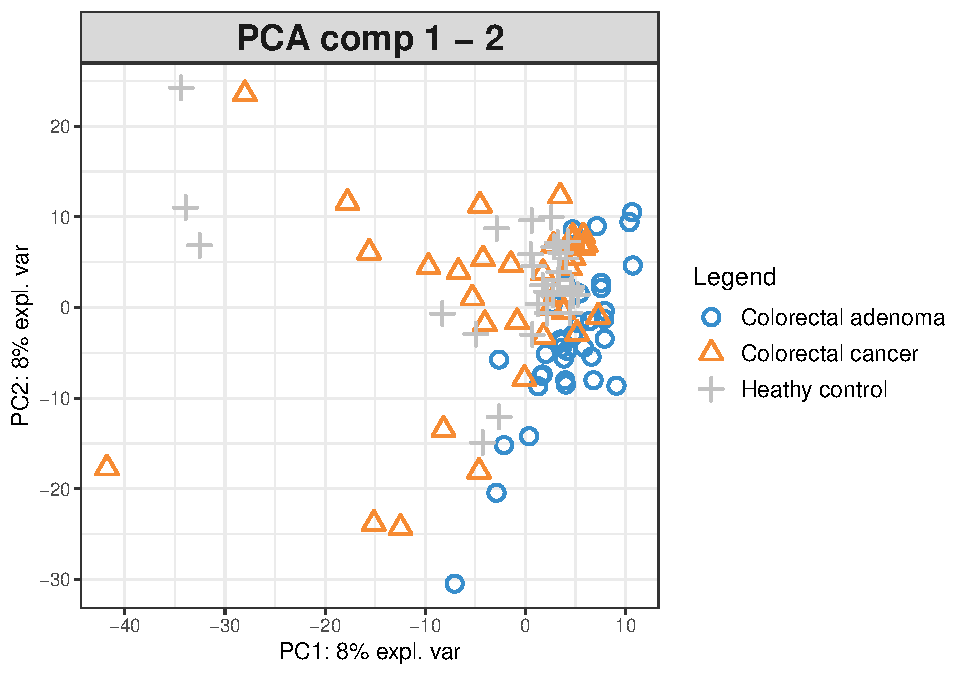
\includegraphics[width=0.6\linewidth]{Getino-Alvarez-Lidia-PEC1_files/figure-latex/PCA Analysis-1} \end{center}

Como se puede observar, a penas existe separación entre los distintos
grupos y el porcentaje de variabilidad explicado por las dos primeras
componentes es bastante bajo. Esto pone de manifiesto que, a priori, no
hay diferencias metabólicas claras entre los distintos grupos de
pacientes. Sin embargo, se procede con el PLS-DA que, al ser un método
supervisado, permitirá una mayor discriminación de los grupos por su
perfil metabólico.

\begin{Shaded}
\begin{Highlighting}[]
\CommentTok{\# Aplico PLS{-}DA partiendo de un numero elevado de componentes, 10, para luego}
\CommentTok{\# realizar una validación del número óptimo de componentes}
\NormalTok{plsda }\OtherTok{\textless{}{-}} \FunctionTok{plsda}\NormalTok{(X,Y, }\AttributeTok{ncomp =} \DecValTok{10}\NormalTok{)}

\CommentTok{\# Llevo a cabo la validación aplicando el método de validación cruzada k{-}fold}
\FunctionTok{set.seed}\NormalTok{(}\DecValTok{123}\NormalTok{)}
\NormalTok{perf.plsda }\OtherTok{\textless{}{-}} \FunctionTok{perf}\NormalTok{(plsda, }\AttributeTok{validation =} \StringTok{\textquotesingle{}Mfold\textquotesingle{}}\NormalTok{, }\AttributeTok{folds =} \DecValTok{3}\NormalTok{,}
                   \AttributeTok{nrepeat =} \DecValTok{50}\NormalTok{)}

\FunctionTok{plot}\NormalTok{(perf.plsda, }\AttributeTok{sd =} \ConstantTok{TRUE}\NormalTok{, }\AttributeTok{legend.position =} \StringTok{"horizontal"}\NormalTok{)}
\end{Highlighting}
\end{Shaded}

\begin{center}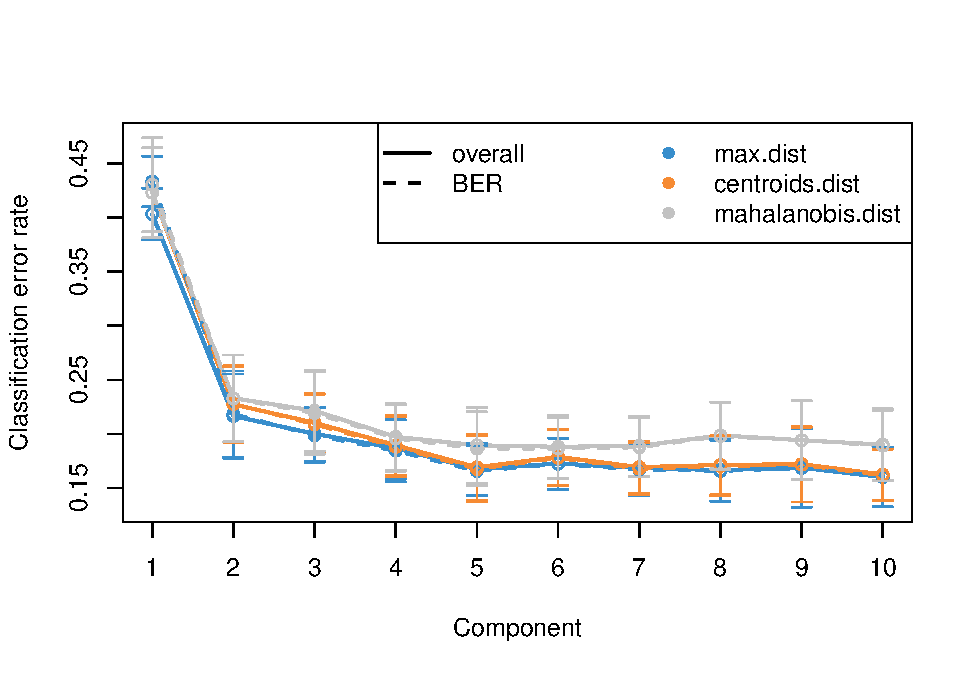
\includegraphics[width=0.7\linewidth]{Getino-Alvarez-Lidia-PEC1_files/figure-latex/PLS-DA ncomp selection-1} \end{center}

En la gráfica del rendimiento de clasificación, se observa que la tasa
de error disminuye notablemente entre la primera y la segunda
componente. A partir de ese punto, disminuye ligeramente alcanzando un
mínimo en la quinta componente. Sin embargo, se seleccionan las dos
primeras componentes para evitar un posible error de sobreajuste.

\begin{Shaded}
\begin{Highlighting}[]
\CommentTok{\# Re{-}aplico el PLS{-}DA con el número de componentes seleccionado}
\NormalTok{plsda }\OtherTok{\textless{}{-}} \FunctionTok{plsda}\NormalTok{(X,Y, }\AttributeTok{ncomp =} \DecValTok{2}\NormalTok{)}

\CommentTok{\# Ploteo los resultados}
\FunctionTok{plotIndiv}\NormalTok{(plsda,}
          \AttributeTok{ind.names =} \ConstantTok{FALSE}\NormalTok{,}
          \AttributeTok{legend =} \ConstantTok{TRUE}\NormalTok{,}
          \AttributeTok{ellipse =} \ConstantTok{TRUE}\NormalTok{, }
          \AttributeTok{title =} \StringTok{"PLS{-}DA comp 1{-}2"}\NormalTok{,}
          \AttributeTok{X.label =} \StringTok{\textquotesingle{}PLS{-}DA comp 1\textquotesingle{}}\NormalTok{, }\AttributeTok{Y.label =} \StringTok{\textquotesingle{}PLS{-}DA comp 2\textquotesingle{}}\NormalTok{)}
\end{Highlighting}
\end{Shaded}

\begin{center}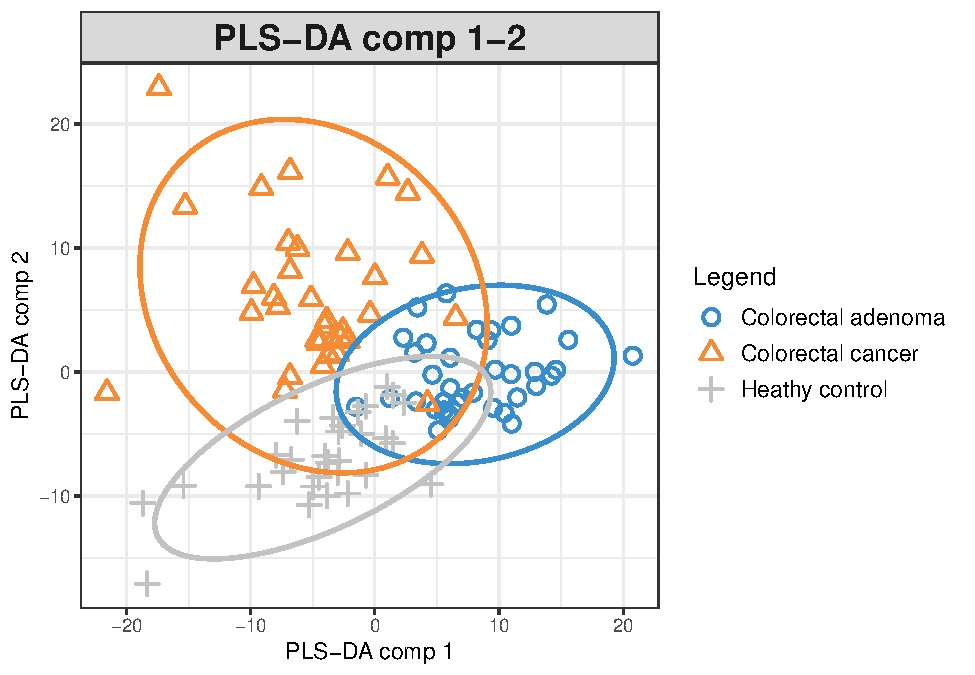
\includegraphics[width=0.6\linewidth]{Getino-Alvarez-Lidia-PEC1_files/figure-latex/PLS-DA-1} \end{center}

Tras la aplicación de un método supervisado, como es el PLS-DA, se
observa una mejor agrupación de los datos en función del grupo al que
pertenecen los pacientes. Sin embargo, se sigue observando bastante
solapamiento entre los grupos, sugiriendo que, aunque hay perfiles
metabólicos distintivos, estos no proporcionan una separación clara.

\begin{Shaded}
\begin{Highlighting}[]
\CommentTok{\# Aplico de nuevo el método de validación cruzada k{-}fold sobre el PLS{-}DA final}
\FunctionTok{set.seed}\NormalTok{(}\DecValTok{123}\NormalTok{)}
\NormalTok{perf.plsda }\OtherTok{\textless{}{-}} \FunctionTok{perf}\NormalTok{(plsda, }\AttributeTok{validation =} \StringTok{\textquotesingle{}Mfold\textquotesingle{}}\NormalTok{, }\AttributeTok{folds =} \DecValTok{3}\NormalTok{,}
                   \AttributeTok{nrepeat =} \DecValTok{50}\NormalTok{)}

\CommentTok{\# Muestro la tasa de error por clase en cada componente}
\NormalTok{perf.plsda}\SpecialCharTok{$}\NormalTok{error.rate.class}\SpecialCharTok{$}\NormalTok{max.dist}
\end{Highlighting}
\end{Shaded}

\begin{verbatim}
##                         comp1     comp2
## Colorectal adenoma  0.0600000 0.1578378
## Colorectal cancer   0.3405714 0.2668571
## Heathy control      0.9000000 0.2300000
\end{verbatim}

A partir de este resultado, se puede observar que la primera componente
tiende a clasificar muy adecuadamente a los pacientes de adenoma
colorectal, mientras que tiene una elevada tasa de error a la hora de
clasificar a los pacientes control. Al incluir la segunda componente,
sin embargo, observamos como las tasas de error se equilibran
notablemente entre los tres grupos, siendo más adecuado para el objetivo
deseado.

Las tasas de error obtenidas con la segunda componente se encuentran en
todos los casos por debajo del 30\%, reforzando lo que se observaba en
el gráfico previo: se podría considerar que sí existen perfiles
metabólicos distintivos entre los tres grupos, aunque estos no
proporcionan una separación perfecta de los mismos.

\section{4. Discusión y conclusiones}\label{discusiuxf3n-y-conclusiones}

El conjunto de datos seleccionado ha resultado de gran versatilidad a la
hora de realizar los ejercicios propuestos. La presencia de varios
ensayos (\emph{assay}), así como de sus respectivos metadatos, han
permitido enriquecer el proceso de exploración e interacción con los
datos.

A la hora de realizar el análisis estadístico con PLS-DA, se tomó la
decisión de emplear sólo uno de los dos ensayos disponibles, con el fin
de mantener el informe conciso. Sin embargo, esto ha limitado la
capacidad de responder a la pregunta biológica planteada. Sería
interesante ampliar el estudio realizando también el análisis
estadístico sobre los datos del segundo ensayo e, incluso, se podría
valorar la opción de unificar ambos conjuntos, teniendo en cuenta que
los metabolitos detectados en cada uno de los ensayos son completamente
diferentes entre sí y no habría riesgo de duplicados. Esta integración
podría proporcionar una imagen más completa de los perfiles metabólicos
de cada grupo y de las potenciales diferencias entre ellos.

\section{\texorpdfstring{5. URL del respositorio de
\emph{github}}{5. URL del respositorio de github}}\label{url-del-respositorio-de-github}

La \textbf{URL} del respositorio público de \emph{github} en el que se
pueden localizar tanto el presente informe, como todos los archivos
asociados a este, es:
\url{https://github.com/lidiaga/Getino-Alvarez-Lidia-PEC1}

\renewcommand\refname{6. Bibliografía}
  \bibliography{PEC1bib.bib}

\end{document}
